\begin{prob}
    Suppose the Bellman-Ford algorithm with early stopping is run on the
    weighted graph shown below using node $s$ as the source (the edge weights are
    intentionally not shown). In the worst case, how many iterations of Bellman-Ford will
    be performed? That is, how many iterations of the outer \python{for}-loop will
    occur?

    \begin{center} 
        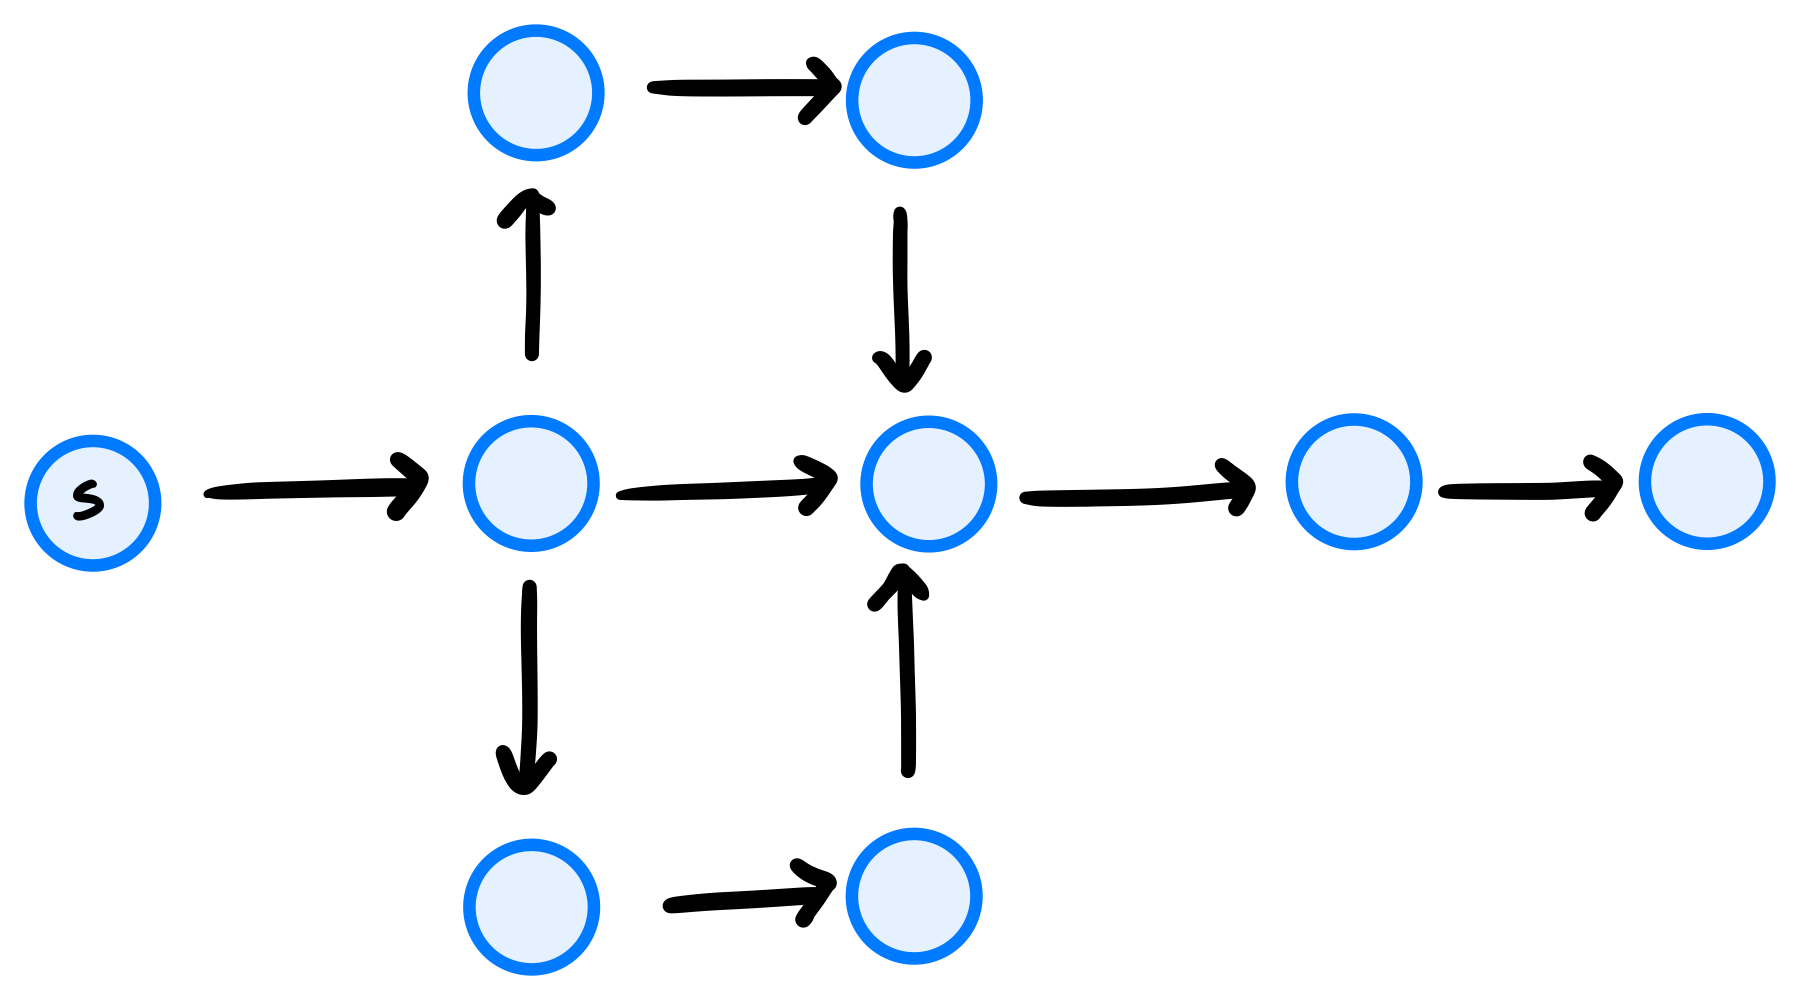
\includegraphics[width=.6\textwidth]{./fig/g6.png}
    \end{center}

    \inlineresponsebox[1.5in]{7}

\end{prob}
